\hypertarget{highly-overlapped-signals}{%
\chapter{Highly Overlapped Signals}\label{highly-overlapped-signals}}

In the previous chapter, I introduced basic signal processing fundamentals in the context of audio mixtures.
In this chapter I want to focus on scenarios of highly overlapped signals.
In order to make an attempt to formalize these, I start with a recap of time-frequency representations as introduced in Section~\ref{sub:time-frequency-representation} and how they are typically applied to address the source separation problem.

\hypertarget{separability-of-mixtures}{%
\section{Separability of Mixtures}\label{separability-of-mixtures}}

TF representations have obvious benefits such as the improved interpretability due to its ``image-like'' two-dimensional properties.
But more importantly, such a representation is very suitable to separate mixtures of speech and musical instruments.
The reason for this is that these mixtures may be fully overlapped in the time domain but are less overlapped in the frequency domain~\cite{rickard02, giannoulis11, rafii}.
% still minor relation to rafii, but seems ok
In turn, a TF representation allows to apply filtering in a way that sufficiently extracts all targets from the mixture.
Furthermore, it allows for simple reconstruction of the original waveform and provides a good trade-off between computational complexity and separation quality.
\par
Due to these reasons many source separation methods focus on extracting individual sources by modeling their respective target in the time-frequency domain.
% check
It is a reasonable approach where it is usually assumed that the time-frequency-domain (STFT) provides sufficient level of separability (e.g.~by given a perfect mask).
The actual extraction or filtering is done by synthesizing the magnitude estimate of the model and applying the originals mixture phase.
\par
In practice, the ability to extract a source from a mixture, depends on the amount of overlap between sources.
Without any overlap, separation is not necessary, and a small amount of overlap can be tolerated to still sufficiently extract the sources.
However, if sources are fully overlapped in both, time and frequency, a separation in the TF domain is hardly possible.
This property, called \emph{separability}, was found by Rickard in~\cite{rickard02} and a useful metric for both, speech and music~\cite{giannoulis11} signals.
\par
% check
In linear mixtures, separability is defined as \emph{a measure that indicates the percentage of time-frequency bins of a source is disjoint from those of interfering sources}.
If \(M\) is the ideal binary mask for a given target \(S\) and it's interfering
magnitude model \(Y\), \(WDO\) is defined as:

\begin{equation}
    PSR_{M} = \frac{\|M \cdot S_{k}\|^{2}}{\|S_{k}\|^{2}}
\end{equation}

\begin{equation}
    SIR_{M}=\frac{\|M \cdot S_{k}\|^{2}}{\|M \cdot Y_{k}\|^{2}}
\end{equation}

\begin{equation}
    WDO_{M} = PSR_{M} - \frac{PSR_{M}}{SIR_{M}}
\end{equation}

%Ideal Ratio Mask:
%\(\hat{\mathbf{x}}=\frac{\mathbf{v_j}}{\sum_{j'=1}^{J}\mathbf{v}_j'}\mathbf{x}\)

A \(WDO\) of one means the sources are perfectly disjoint, hence no overlap.
A \(WDO\) zero means can be interpreted as sources being fully overlapped.
An extensive study using this W-disjoint orthogonality metric (WDO) is given in~\cite{rickard02}.
\par
Research on mixtures is often focused on specific, application-driven scenarios to analyze and separate mixtures.
I want to focus on two scenarios that remain very popular among research with a large amount of contributions:

\begin{description}
  \item[Cocktail Party] where multiple speakers are active at the same time (concurrent).
  Due to the fact that concurrent speakers are speaking at the same time, it results in an overlap of speech signals in both time an frequency.
  \item[Vocals and Accompaniment] are usually present at the same time in professionally produce music. 
  Often, the main assumption is that vocals are more sparse, whereas the accompaniment is more stationary.
\end{description}

Now, for both scenarios, the actual overlap is dependent on additional parameters like the the number of sources, the class of source or the fundamental frequency.
For instance, the overlap in a cocktail party of two speakers is smaller than with ten concurrent speakers speaking.
Also the overlap between male and female or brass and string instruments is smaller than with two instruments of the same class. 
And if two instrumental notes share the same fundamental frequency (playing in \emph{unison}), the sources are almost completely overlapped.
\par
\begin{figure*}[h]
\centering
\subcaptionbox[Speech]{Speech}%
[1\textwidth]{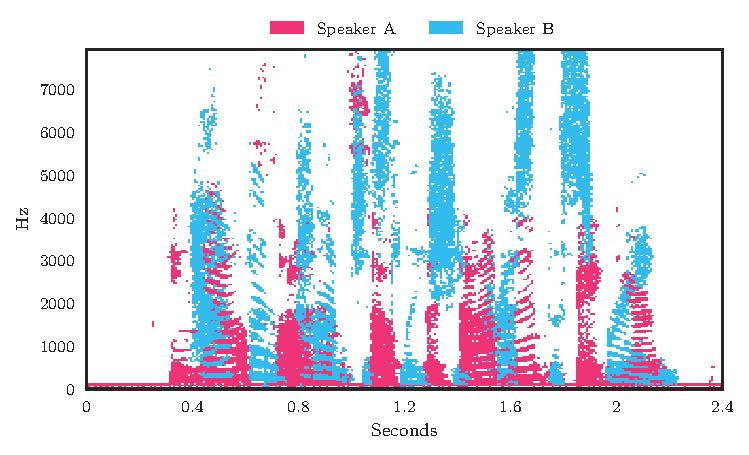
\includegraphics[width=0.8\textwidth]{gfx/dominance_map_speakers.pdf}}%
\hspace{0.2\textwidth} % seperation
\subcaptionbox[Vocal/Accompaniment]{Vocal/Accompaniment}
[1\textwidth]{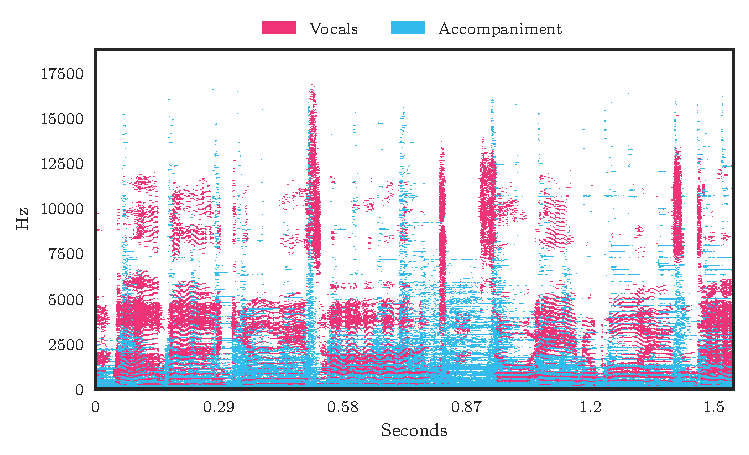
\includegraphics[width=0.8\textwidth]{gfx/dominance_map_vocacc.pdf}}%
\hspace{0.2\textwidth} % seperation
\subcaptionbox[Speech]{Unsison}
[1\textwidth]{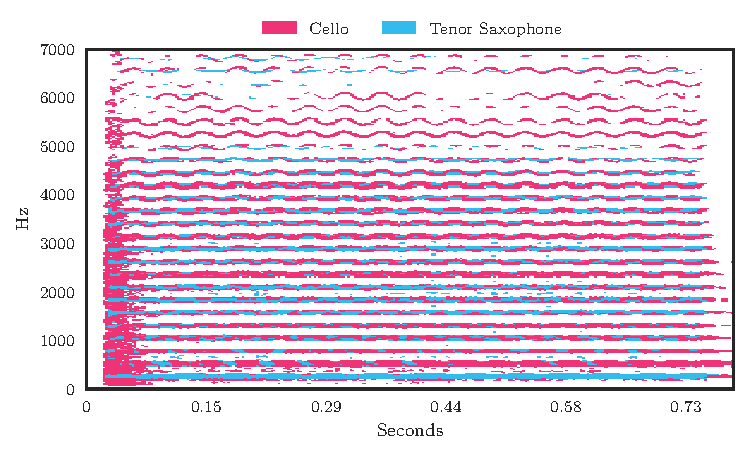
\includegraphics[width=0.8\textwidth]{gfx/dominance_map_unison.pdf}}%
\caption{Predominant source activity, showing the predominant source for each time frequency entry. Computed using binary masks of each source entry.}
\label{fig:dominance}
\end{figure*}

\begin{figure*}[h]
\centering
\subcaptionbox[Speech]{Speech}%
[1\textwidth]{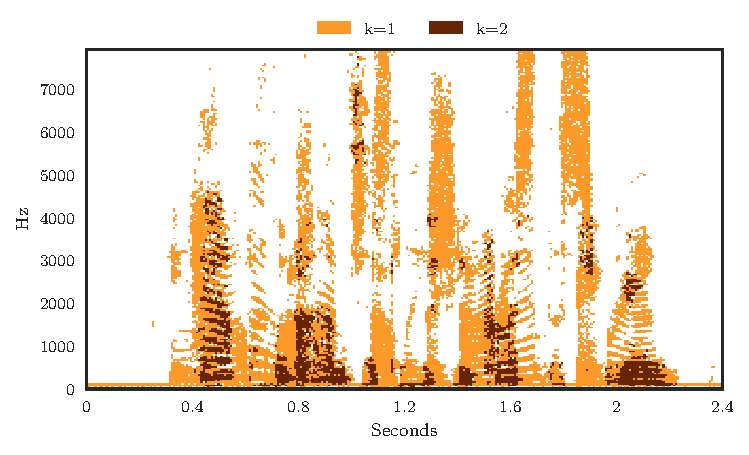
\includegraphics[width=0.8\textwidth]{gfx/count_map_speakers.pdf}}%
\hspace{0.2\textwidth} % seperation
\subcaptionbox[Vocal/Accompaniment]{Vocal/Accompaniment}
[1\textwidth]{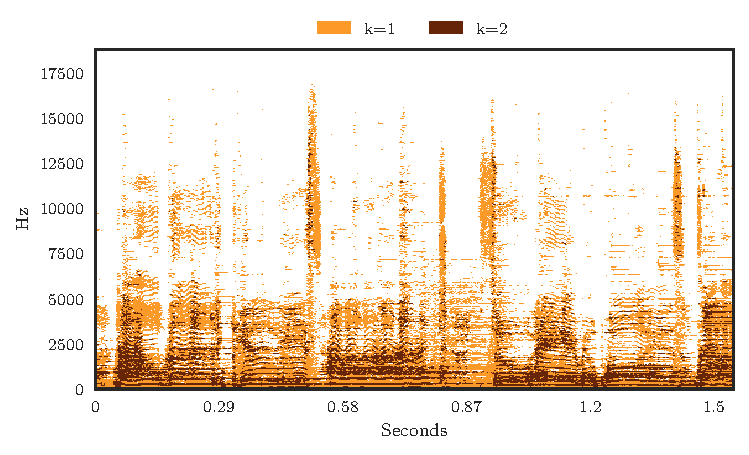
\includegraphics[width=0.8\textwidth]{gfx/count_map_vocacc.pdf}}%
\hspace{0.2\textwidth} % seperation
\subcaptionbox[Unison]{Unison Instruments}
[1\textwidth]{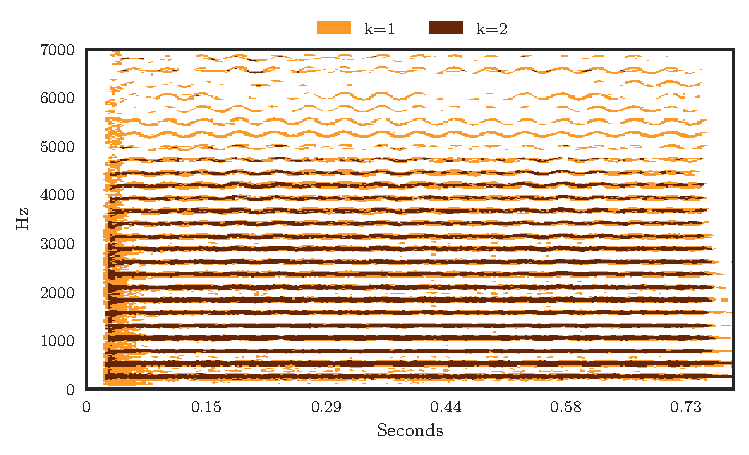
\includegraphics[width=0.8\textwidth]{gfx/count_map_unison.pdf}}%
\caption{Source Count Activity showing the number of sources $k$ for each time frequency entry. Computed using binary masks of each source entry.}
\label{fig:count}
\end{figure*}

To illustrate this, I depict the different scenarios in Figures~\ref{fig:dominance} and~\ref{fig:count}.
The Figure~\ref{fig:dominance} shows the number of TF entries that predominantly belong to either one of the two source classes.
Figure~\ref{fig:count} shows the number of active sources of each TF entry for the same audio signals.
From these figures, one can see that the overlap of a typical speech mixture is comparable to a music recording where the task is to separate vocals and accompaniment.
If we now compare this to the scenario where sources are fully overlapped as in the unison scenario, almost all TF bins are overlapped and separation would hardly be possible.
\par
While this is an extreme scenario, it provides a case where typical assumptions are violated and it would facilitate the demand to develop new methods that do not rely so much on these long standing assumptions.
To come up with an idea for a method that could successfully separate unison case is possible by just observing closely the spectrograms of Figure~\ref{fig:count}.
We see that the slow spectro-temporal modulations caused by the vibratos is one of the aspects where the two sources differ significantly.
So instead of a TF representation, one would need to pick a representation that allows to separate the two sources in their modulation domain.
Therefore, I want to focus on these ``modulational'' aspects on mixtures in the next section.

\hypertarget{utilizing-slow-modulations}{%
\section{Utilizing Slow Modulation}\label{utilizing-slow-modulations}}

Slowly varying tempo-spectral modulations occur both in speech and music signals and are a combination between amplitude and frequency modulation (See introduction in Section~\ref{sub:time-variant-audio-signals}).

% Steps: 
% 1. analyse the cause of fluctuation
% 2. analyze the target (mix)

\subsection{Analysis}
In music, vibrato is an effect that is well studied especially in musicology~\cite{A, B, C, D, E}.
Performers of musical to perform a vibrato in the same way when repeating a performance. This can be exploited in
source separation scenarios.
Typically, vibratos have modulation frequencies (rates) which vary between 4 and 8 Hz which is magnitudes slower compare to the actual fundamental frequency of the source.
Additionally vibrato rates vary across different instruments.
In~\cite{macleod2006} the vibrato width (frequency deviation) was found to be significantly different between violinists and violists performers.\\

\subsection{Perception}
There are indications that humans use modulations to segregate sounds as well~\cite{dau99}.
Humans make use of the concept of Common Amplitude Modulation~\cite{bregman90} to segregate sources in mixture.
CAM is effectively the property of harmonics that share the
same amplitude modulation across the bins.

% The upper limit of modulation detection extends to 2.2 kHz

% <20Hz -> ~\cite{schreiner88}

% \cite{zwicker52, plomp93, fastl90}

% General psychoacoustic theory: \cite{bregman}

Humans use amplitude modulation for their common grouping procedure.

> ~\cite{dau99}: It appears that the auditory system is very sensitive to slow modulations. Slow modulations are associated with the perception of rhythm. Samples of running speech, for example, show distributions of modulation frequencies with peaks around 3-4 Hz, approximately corresponding to the sequence rate of syllables (Plomp, 1983). Results from physiological studies have shown that, at least in mammals, the auditory cortex seems to be limited in its ability to follow fast temporal changes.

depending on the carrier frequency and the modulation frequency, humans describe modulations differently as fluctuation, roughness, or residue pitch (See Figure 2 in~\cite{joris04}).

~\cite{bacon89, dau99} showed that human perceptual limits of amplitude modulations can be modeled...

~\cite{mcadams89} showed that modulation cues are used to group sounds. 
--> Common fate

--> challanges

* tracking modulations is hard, because f0 estimation doesn't easily work on mixtures. Reason is that crossing partials is a big problem for sinusoidal modeling~\cite{viste03}

* modulations are not present in all signal types. so you need to be lucky 
* Papers with detecting vibrato?
* Representations are not easily invertible

~\cite{scheirer99}
> technique  operates  by  discovering  common  modulation  behavior among groups of frequency subbands in the autocorrelogram domain.  

\subsection{Representations}
One way of analyzing amplitude modulations is to use a modulation spectrogram~\cite{greenberg97} which is a frequency-frequency
representation of a time domain input signal.
A complete signal representation can be archived by a modulation tensor which holds the modulation spectrograms for each time frame.
For further details the reader is referred to~\cite{barker15}.

\subsection{Processing}
There exist a number of method that utilise spectro-temporal modulation to process or separate mixtures.

~\cite{creager16} VibratoNTF uses DOA 

~\cite{li09}, exploitung common amplitude modulation for source separation

\cite{viste03}
\begin{quote}
harmonic relation, the common onset, offset, amplitude modulation (AM), and frequency modulation (FM).These are all important cues for grouping.  
\end{quote}

%lets start with speech
In speech, techniques to utilize modulation patterns enabled applications such as~\cite{mesgarani04} or extract spatial acoustic signatures from mixtures~\cite{sukittanon06}.
Is also shown that it can improve speech intelligibility~\cite{elhilali03} or automatic speech recognition~\cite{kingsbury98}.

% from zafar!
Wang proposed instantaneous and frequency-warped techniques for signal parameterization and source separation, with application to voice separation in music~\cite{wang94,wang95}.
He introduced a frequency-locked loop algorithm which uses multiple harmonically constrained trackers.
He computed the estimated fundamental frequency from a maximum-likelihood weighting of the tracking estimates. He was then able to estimate harmonic signals such as voices from complex mixtures.\\
% from zafar
Wolf et al. proposed an approach using rigid motion segmentation, with application to singing voice separation \cite{wolf14,wolf16}. They introduced harmonic template models with amplitude and pitch modulations defined by a velocity vector. They applied a wavelet transform \cite{anden14} on the harmonic template models to build an audio image where the amplitude and pitch dynamics can be separated through the velocity vector. They then derived a velocity equation, similar to the optical flow velocity equation used in images \cite{bernard01}, to segment velocity components. Finally, they identified the harmonic templates which model different sources in the mixture and separated them by approximating the velocity field over the corresponding harmonic template models.\\
% from zafar
Yen et al. proposed an approach using spectro-temporal modulation features \cite{yen14,yen15}. They decomposed a mixture using a two-stage auditory model which consists of a cochlear module \cite{chi05} and cortical module \cite{chi99}. They then extracted spectro-temporal modulation features from the TF units and clustered the TF units into harmonic, percussive, and vocal components using the EM algorithm and resynthesized the estimated signals.\\
% from zafar
% double check this!
Virtanen made us of sinuoidal modeling \cite{virtanen00} to model and separate sources with tempo spectral modulation like vibrato.

Usage for source separation, non FM modulations are considered: \cite{hennequin10}.
An advantage of the source-filter model approach is indeed that one can dissociate the pitched content of the signal, embodied by the position of its harmonics, from its TF envelope which describes where the energy of the sound lies. In the case of vocals, it yields the ability to distinguish between the actual note being sung (pitch content) and the phoneme being uttered (mouth and vocal tract configuration), respectively. One key feature of vocals is they typically exhibit great variability in fundamental frequency over time. They can also exhibit larger \textit{vibratos} (fundamental frequency modulations) and \textit{tremolos} (amplitude modulations) in comparison to other instruments.

% from zafar
The concept of \emph{common amplitude modulation} by~\cite{bregman, wang06} which exploits that amplitude envelopes of different harmonics of the same source tend to be similar.
Modeling the common amplitude modulation to separate mixtures has already been done in~\cite{li07} and \cite{cano14}, which additionally included common amplitude modulation characteristics in the separation scheme.

separating without understanding

> ~\cite{greenberg96} the energy in the modulation spectrum may be derived from syllabic segmentation. This association is of interest in light of recent demonstrations that speech intelligibility is crucially dependent on the preservation of the portion of the modulation spectrum between 2 and 10 Hz

\section{Summary and Discussion}

% TODO: add deep learning

% TODO: the gap

% summary (mini objectives)
Highly overlapped signals require suitable representations, because separability is of highly overlapped source with modulations is sufficiently possible in the TF domain.

Many of the representations require a parametric approach. And the existing modulation tensor is only able to capture amplitude modulation, hence it cannot solve general modulations.

\begin{itemize}
  \item What is the likeliness for two target signals being overlapped for different scenarios
  \item Unison
  \item past research was focused on solving source separation because its such an interesting and challenging mathematical problem. Data driven separation, however, changed this.
\end{itemize}
